\begin{enumerate}[label=\thesection.\arabic*,ref=\thesection.\theenumi]
\item Find the sum of the vectors $\vec{a}=\hat{i}-2\hat{j}+\hat{k}$, $\vec{b}=-2\hat{i}+4\hat{j}+5\hat{k}$ and $\vec{c}=\hat{i}-6\hat{j}-7\hat{k}$.
\item 

	In triangle ABC (Fig 10.18), which of the following is not true:
 \begin{enumerate}
         \item $\overrightarrow{AB}+\overrightarrow{BC}+\overrightarrow{CA}$=$\vec{0}$
         \item $\overrightarrow{AB}+\overrightarrow{BC}-\overrightarrow{CA}$=$\vec{0}$
         \item $\overrightarrow{AB}+\overrightarrow{BC}-\overrightarrow{CA}$=$\vec{0}$
         \item $\overrightarrow{AB}-\overrightarrow{BC}+\overrightarrow{CA}$=$\vec{0}$
\end{enumerate}
\begin{figure}[h]
\centering
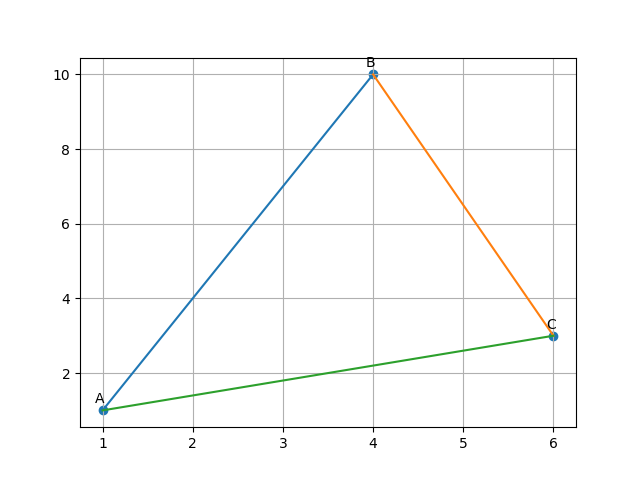
\includegraphics[width = \columnwidth]{./chapters/12/10/2/18/figs/triangle.png}
\caption{}
	\label{fig:chapters/12/10/2/18/}
\end{figure}
\solution
		\iffalse
\documentclass[journal,12pt,twocolumn]{IEEEtran}
\usepackage{romannum}
\usepackage{float}
\usepackage{setspace}
\usepackage{gensymb}
\singlespacing
\usepackage[cmex10]{amsmath}
\usepackage{amsthm}
\usepackage{mathrsfs}
\usepackage{txfonts}
\usepackage{stfloats}
\usepackage{bm}
\usepackage{cite}
\usepackage{cases}
\usepackage{subfig}
\usepackage{longtable}
\usepackage{multirow}
\usepackage{enumitem}
\usepackage{mathtools}
\usepackage{steinmetz}
\usepackage{tikz}
\usepackage{circuitikz}
\usepackage{verbatim}
\usepackage{tfrupee}
\usepackage[breaklinks=true]{hyperref}
\usepackage{tkz-euclide}
\usetikzlibrary{calc,math}
\usepackage{listings}
    \usepackage{color}                                            %%
    \usepackage{array}                                            %%
    \usepackage{longtable}                                        %%
    \usepackage{calc}                                             %%
    \usepackage{multirow}                                         %%
    \usepackage{hhline}                                           %%
    \usepackage{ifthen}                                           %%
  %optionally (for landscape tables embedded in another document): %%
    \usepackage{lscape}     
\usepackage{multicol}
\usepackage{chngcntr}
\DeclareMathOperator*{\Res}{Res}
\renewcommand\thesection{\arabic{section}}
\renewcommand\thesubsection{\thesection.\arabic{subsection}}
\renewcommand\thesubsubsection{\thesubsection.\arabic{subsubsection}}

\renewcommand\thesectiondis{\arabic{section}}
\renewcommand\thesubsectiondis{\thesectiondis.\arabic{subsection}}
\renewcommand\thesubsubsectiondis{\thesubsectiondis.\arabic{subsubsection}}

% correct bad hyphenation here
\hyphenation{op-tical net-works semi-conduc-tor}
\def\inputGnumericTable{}                                 %%

\lstset{
frame=single, 
breaklines=true,
columns=fullflexible
}

\begin{document}


\newtheorem{theorem}{Theorem}[section]
\newtheorem{problem}{Problem}
\newtheorem{proposition}{Proposition}[section]
\newtheorem{lemma}{Lemma}[section]
\newtheorem{corollary}[theorem]{Corollary}
\newtheorem{example}{Example}[section]
\newtheorem{definition}[problem]{Definition}
\newcommand{\BEQA}{\begin{eqnarray}}
\newcommand{\EEQA}{\end{eqnarray}}
\newcommand{\define}{\stackrel{\triangle}{=}}

\bibliographystyle{IEEEtran}
\providecommand{\mbf}{\mathbf}
\providecommand{\pr}[1]{\ensuremath{\Pr\left(#1\right)}}
\providecommand{\qfunc}[1]{\ensuremath{Q\left(#1\right)}}
\providecommand{\sbrak}[1]{\ensuremath{{}\left[#1\right]}}
\providecommand{\lsbrak}[1]{\ensuremath{{}\left[#1\right.}}
\providecommand{\rsbrak}[1]{\ensuremath{{}\left.#1\right]}}
\providecommand{\brak}[1]{\ensuremath{\left(#1\right)}}
\providecommand{\lbrak}[1]{\ensuremath{\left(#1\right.}}
\providecommand{\rbrak}[1]{\ensuremath{\left.#1\right)}}
\providecommand{\cbrak}[1]{\ensuremath{\left\{#1\right\}}}
\providecommand{\lcbrak}[1]{\ensuremath{\left\{#1\right.}}
\providecommand{\rcbrak}[1]{\ensuremath{\left.#1\right\}}}
\theoremstyle{remark}
\newtheorem{rem}{Remark}
\newcommand{\sgn}{\mathop{\mathrm{sgn}}}
\providecommand{\abs}[1]{\left\vert#1\right\vert}
\providecommand{\res}[1]{\Res\displaylimits_{#1}} 
\providecommand{\norm}[1]{\left\lVert#1\right\rVert}
\providecommand{\mtx}[1]{\mathbf{#1}}
\providecommand{\mean}[1]{E\left[ #1 \right]}
\providecommand{\fourier}{\overset{\mathcal{F}}{ \rightleftharpoons}}
\providecommand{\system}{\overset{\mathcal{H}}{ \longleftrightarrow}}
\newcommand{\solution}{\noindent \textbf{Solution: }}
\newcommand{\cosec}{\,\text{cosec}\,}
\providecommand{\dec}[2]{\ensuremath{\overset{#1}{\underset{#2}{\gtrless}}}}
\newcommand{\myvec}[1]{\ensuremath{\begin{pmatrix}#1\end{pmatrix}}}
\newcommand{\mydet}[1]{\ensuremath{\begin{vmatrix}#1\end{vmatrix}}}
\numberwithin{equation}{subsection}
\makeatletter
\@addtoreset{figure}{problem}
\makeatother

\let\StandardTheFigure\thefigure
\let\vec\mathbf
\renewcommand{\thefigure}{\theproblem}



\def\putbox#1#2#3{\makebox[0in][l]{\makebox[#1][l]{}\raisebox{\baselineskip}[0in][0in]{\raisebox{#2}[0in][0in]{#3}}}}
     \def\rightbox#1{\makebox[0in][r]{#1}}
     \def\centbox#1{\makebox[0in]{#1}}
     \def\topbox#1{\raisebox{-\baselineskip}[0in][0in]{#1}}
     \def\midbox#1{\raisebox{-0.5\baselineskip}[0in][0in]{#1}}

\vspace{3cm}


\title{Assignment 1}
\author{Jaswanth Chowdary Madala}





% make the title area
\maketitle

\newpage

%\tableofcontents

\bigskip

\renewcommand{\thefigure}{\theenumi}
\renewcommand{\thetable}{\theenumi}

\begin{enumerate}
\item In the following figure for the triangle ABC, which of the following is not true:

(A) $\overrightarrow{AB}+\overrightarrow{BC}+\overrightarrow{CA} = \overrightarrow{0}$

(B) $\overrightarrow{AB}+\overrightarrow{BC}-\overrightarrow{AC} = \overrightarrow{0}$

(C) $\overrightarrow{AB}+\overrightarrow{BC}+\overrightarrow{AC} = \overrightarrow{0}$

(D) $\overrightarrow{AB}-\overrightarrow{CB}+\overrightarrow{CA} = \overrightarrow{0}$

\textbf{Solution:}
\fi
		We know that,
\begin{align}
\overrightarrow{AB} = \vec{B} - \vec{A}\\
\overrightarrow{BC} = \vec{C} - \vec{B}\\
\overrightarrow{CA} = \vec{A} - \vec{C}
\end{align}
By usinig this we verify each of the given option

\begin{enumerate}
\item 
\begin{align}
\overrightarrow{AB}+\overrightarrow{BC}+\overrightarrow{CA} &=
\vec{B}-\vec{A} + \vec{C} - \vec{B} + \vec{A} - \vec{C}\\
 &= 0
\end{align}
Option A is correct.

\item
\begin{align}
\overrightarrow{AB}+\overrightarrow{BC}-\overrightarrow{AC} &=
\vec{B}-\vec{A} + \vec{C} - \vec{B} - (\vec{C} - \vec{A})\\
 &= 0
\end{align}
Option B is correct.

\item 
\begin{align}
\overrightarrow{AB}+\overrightarrow{BC}+\overrightarrow{AC} &=
\vec{B}-\vec{A} + \vec{C} - \vec{B} + \vec{C} - \vec{A}\\
 &= 2(\vec{C}-\vec{A})
\end{align}
Option C is incorrect.

\item
\begin{align}
\overrightarrow{AB}-\overrightarrow{CB}+\overrightarrow{CA} &=
\vec{B}-\vec{A} - (\vec{B} - \vec{C}) + \vec{A} - \vec{C}\\
 &= 0
\end{align}
Option D is correct.
\end{enumerate}
Verification: Let us take an example to verify 
\begin{align}
\vec{A} = \myvec{1\\1}, 
\vec{B} = \myvec{3\\1},
\vec{C} = \myvec{6\\6} \\
\overrightarrow{AB} = \vec{B} - \vec{A} = \myvec{2\\0}, 
\overrightarrow{BC} = \vec{C} - \vec{B} = \myvec{3\\5},
\overrightarrow{CA} = \vec{A} - \vec{C} = \myvec{-5\\-5} 
\end{align}
Thus,
\begin{align}
\overrightarrow{AB}+\overrightarrow{BC}+\overrightarrow{CA} = \myvec{2+3+(-5) \\ 0+5+(-5)} = \myvec{0 \\0}
\end{align}
Similarly other options can be verified.



\item If $\vec{a}$ and $\vec{b}$ are two collinear vectors, then which of the following are incorrect:
\begin{enumerate}
    \item $\vec{b}=\lambda\vec{a},$
 for some scalar $\lambda$
    \item $\vec{a}=\pm\vec{b}$
    \item the respective components of $\vec{a}$ and $\vec{b}$ are not proportiona
    \item both the vectors $\vec{a}$ and $\vec{b}$ have same direction, but different magnitudes.
\end{enumerate}
	\item If a line makes angles $90\degree,135\degree,45\degree$ with x,y and z-axis respectivly. Find its direction cosines.
		\\
		\solution
		\iffalse
\documentclass[journal,12pt,twocolumn]{IEEEtran}
\usepackage{graphicx}
\graphicspath{{./figs/}}{}
\usepackage{amsmath,amssymb,amsfonts,amsthm}
\newcommand{\myvec}[1]{\ensuremath{\begin{pmatrix}#1\end{pmatrix}}}
\providecommand{\norm}[1]{\lVert#1\rVert}
\usepackage{listings}
\usepackage{watermark}
\usepackage{titlesec}
\usepackage{caption}
\usepackage{gensymb}
\newcommand{\mydet}[1]{\ensuremath{\begin{vmatrix}#1\end{vmatrix}}}
\let\vec\mathbf
\lstset{
frame=single, 
breaklines=true,
columns=fullflexible
}
\thiswatermark{\centering \put(0,-105.0){
\includegraphics[scale=0.15]{/sdcard/IITH/vectors/12.11.1.1/figs/logo.png}} }
\title{\mytitle}
\title{
Assignment - 12.11.1.1
}
\author{Surajit Sarka}
\begin{document}
\maketitle
\tableofcontents
\bigskip
\section{\textbf{Problem}}
\section{\textbf{Solution}}
\fi
The direction vector is
\begin{align}
\vec{A}=\myvec{\cos 90^{\circ}\\ \cos 135^{\circ}\\ \cos 45^{\circ}}=\myvec{0\\-\frac{1}{\sqrt{2}}\\ \frac{1}{\sqrt{2}}}
\end{align}

\item A girl walks 4 km towards west, then she walks 3 km in a direction 30$^{\circ}$ east of north and stops. Determine the girl's displacement from her initial point of departure.\\
	\solution
		\iffalse
\documentclass[12pt]{article}
\usepackage{graphicx}
%\documentclass[journal,12pt,twocolumn]{IEEEtran}
\usepackage[none]{hyphenat}
\usepackage{graphicx}
\usepackage{listings}
\usepackage[english]{babel}
\usepackage{graphicx}
\usepackage{caption}
\usepackage[parfill]{parskip}
\usepackage{hyperref}
\usepackage{booktabs}
\usepackage{gensymb}
%\usepackage{setspace}\doublespacing\pagestyle{plain}
\def\inputGnumericTable{}
\usepackage{color}                                            %%
    \usepackage{array}                                            %%
    \usepackage{longtable}                                        %%
    \usepackage{calc}                                             %%
    \usepackage{multirow}                                         %%
    \usepackage{hhline}                                           %%
    \usepackage{ifthen}
\usepackage{array}
\usepackage{amsmath}   % for having text in math mode
\usepackage{parallel,enumitem}
\usepackage{listings}
\lstset{
language=tex,
frame=single,
breaklines=true
}
 
%Following 2 lines were added to remove the blank page at the beginning
\usepackage{atbegshi}% http://ctan.org/pkg/atbegshi
\AtBeginDocument{\AtBeginShipoutNext{\AtBeginShipoutDiscard}}
%
%New macro definitions
\newcommand{\mydet}[1]{\ensuremath{\begin{vmatrix}#1\end{vmatrix}}}
\providecommand{\brak}[1]{\ensuremath{\left(#1\right)}}
\providecommand{\norm}[1]{\left\lVert#1\right\rVert}
\newcommand{\solution}{\noindent \textbf{Solution: }}
\newcommand{\myvec}[1]{\ensuremath{\begin{pmatrix}#1\end{pmatrix}}}
\let\vec\mathbf
\begin{document}
\begin{center}
\enlargethispage{-4cm}
\title{\textbf{vector Algebra}}
\date{\vspace{-5ex}} %Not to print date automatically
\maketitle
\end{center}
\setcounter{page}{1}
\section*{12$^{th}$ Maths - Chapter 10}
This is Problem-3 from Exercise 10.4
\begin{enumerate}
\item A girl walks $4$ km towards west, then she walk $3$ km in a direction $30\degree$ east of north and stops. Determine the girl's displacement from her initial point of departure.

\solution 
\fi
		Let 
\begin{align}
	\vec{A}=\myvec{0\\0},
			\vec{B} -\vec{A}=\myvec{-4\\0},
	 \vec{C}-\vec{B}=\myvec{3\cos{60\degree}\\3\sin{60\degree}}
&=\myvec{\frac{3}{2}\\ \frac{3\sqrt{3}}{2}}
 \end{align}
 By triangle law of vector addition, 
\begin{align}
	\vec{C}-\vec{A} &= \vec{B}-\vec{A}+\vec{C}-\vec{B}\\
 &=\myvec{-4\\0}+\myvec{\frac{3}{2}\\[2pt] \frac{3\sqrt{3}}{2}}
=\myvec{\frac{-5}{2}\\[2pt] \frac{3\sqrt{3}}{2}}
\end{align}
which is the girl's displacement from her initial point of departure 
See Fig. 
\ref{fig:chapters/12/10/5/3Fig1}.
\begin{figure}[!h] 
 \begin{center} 
 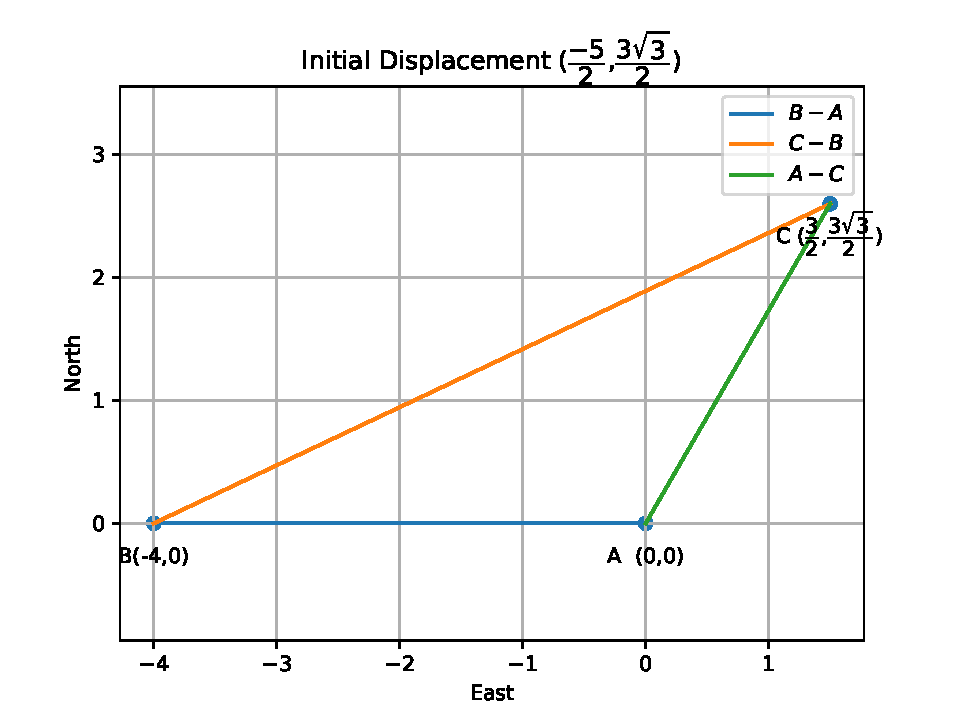
\includegraphics[width=\columnwidth]{chapters/12/10/5/3/figs/fig.pdf} 
 \end{center} 
\caption{} 
\label{fig:chapters/12/10/5/3Fig1} 
\end{figure}

\item If $\vec{a}=\hat{i}+\hat{j}+\hat{k}$,$\vec{b}=2\hat{i}-\hat{j}+3\hat{k}$ and $\vec{c}=\hat{i}-2\hat{j}+\hat{k}$, find a unit vector parallel to the vector $2\vec{a}-\vec{b}+3\vec{c}$.\\
	\solution
		\iffalse
\documentclass[10pt]{article}
\usepackage{graphicx}
\usepackage[none]{hyphenat}
\usepackage{graphicx}
\usepackage{listings}
\usepackage[english]{babel}
\usepackage{siunitx}
\usepackage{graphicx}
\usepackage{caption} 
\usepackage{booktabs}
\usepackage{array}
\usepackage{amssymb} % for \because
\usepackage{amsmath}   % for having text in math mode
\usepackage{extarrows} % for Row operations arrows
\usepackage{listings}
\usepackage[utf8]{inputenc}
\lstset{
  frame=single,
  breaklines=true
}
\usepackage{hyperref}
  
%Following 2 lines were added to remove the blank page at the beginning
\usepackage{atbegshi}% http://ctan.org/pkg/atbegshi
\AtBeginDocument{\AtBeginShipoutNext{\AtBeginShipoutDiscard}}


%New macro definitions
\newcommand{\mydet}[1]{\ensuremath{\begin{vmatrix}#1\end{vmatrix}}}
\providecommand{\brak}[1]{\ensuremath{\left(#1\right)}}
\newcommand{\solution}{\noindent \textbf{Solution: }}
\newcommand{\myvec}[1]{\ensuremath{\begin{pmatrix}#1\end{pmatrix}}}
\providecommand{\norm}[1]{\left\lVert#1\right\rVert}
\providecommand{\abs}[1]{\left\vert#1\right\vert}
\let\vec\mathbf{}
\begin{document}

\begin{center}
\title{\textbf{Vector Algebra}}
\date{\vspace{-5ex}} %Not to print date automatically
\maketitle
\end{center}

\section{12$^{th}$ Maths - Chapter 10}
This is Problem 7 from Exercise-10.5
\begin{enumerate}

\item If $\overrightarrow{a}=\hat{i}+\hat{j}+\hat{k}$,$\overrightarrow{b}=2\hat{i}-\hat{j}+3\hat{k}$ and $\overrightarrow{c}=\hat{i}-2\hat{j}+\hat{k}$, find a unit vector parallel to the vector $2\overrightarrow{a}-\overrightarrow{b}+3\overrightarrow{c}$.\\  

\solution
Given Vectors
\fi

\begin{align}
	\vec{u}=2\vec{a}-\vec{b}+3\vec{c}=\myvec{3\\-3\\2}
\implies
\hat{\vec{u}}=\frac{\vec{u}}{\norm{\vec{u}}}
=\frac{1}{\sqrt{22}}\myvec{3\\-3\\2}
\end{align}


\item The two opposite vertices of a square are $(–1, 2)$  and $ (3, 2)$. Find the coordinates of the other two vertices.
\\
	\iffalse
\documentclass[12pt]{article}
\usepackage{graphicx}
\usepackage{amsmath}
\usepackage{mathtools}
\usepackage{gensymb}

\newcommand{\mydet}[1]{\ensuremath{\begin{vmatrix}#1\end{vmatrix}}}
\providecommand{\brak}[1]{\ensuremath{\left(#1\right)}}
\providecommand{\norm}[1]{\left\lVert#1\right\rVert}
\newcommand{\solution}{\noindent \textbf{Solution: }}
\newcommand{\myvec}[1]{\ensuremath{\begin{pmatrix}#1\end{pmatrix}}}
\let\vec\mathbf

\begin{document}
\begin{center}
\textbf\large{CHAPTER-7 \\ COORDINATE GEOMETRY}

\end{center}
\section*{Excercise 7.4}

Q4.The two opposite vertices of a square are $(–1, 2) \text{ and } (3, 2)$. Find the coordinates of the other two vertices.\\
\fi
\solution
Let
\begin{align}
\vec{A} = \myvec
{
-1 \\
 2\\
},
\vec{C} = 
\myvec
{
3\\
2\\
}
\end{align}

\begin{figure}[!h]
	\begin{center} 
	    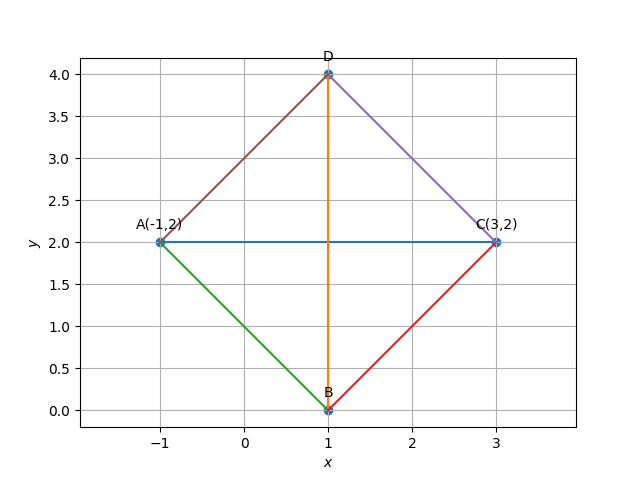
\includegraphics[width=\columnwidth]{chapters/10/7/4/4/figs/square}
	\end{center}
\caption{}
\label{fig:7/4/4/4Fig1}
\end{figure}

Shifting $\vec{A}$ to origin with reference to Fig. \ref{fig:7/4/4/4Fig2},
\begin{align}
\vec{A^{\prime}} =
\myvec{
0 \\
0\\
},
\vec{C^{\prime}} = \vec{C}-\vec{A} = 
\myvec{
4 \\
0\\
}
\end{align}

\begin{figure}[!h]
	\begin{center} 
	    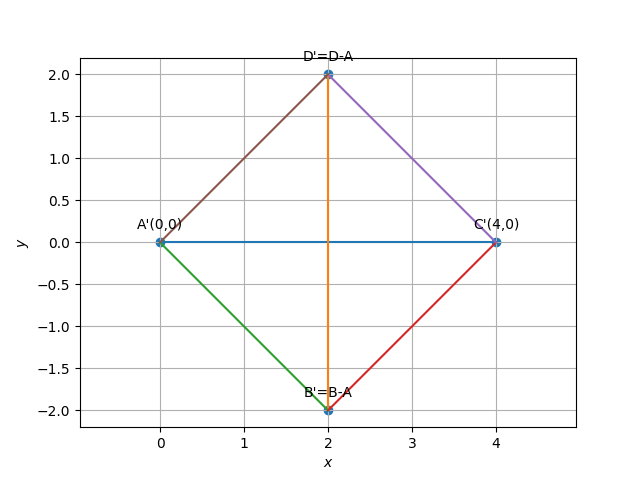
\includegraphics[width=\columnwidth]{chapters/10/7/4/4/figs/square1}
	\end{center}
\caption{}
\label{fig:7/4/4/4Fig2}
\end{figure}
\iffalse
In general,
the angle made by $AC$ with the x-axis is 
		\begin{align}
\beta = \theta + 45\degree
		\end{align}
\fi
Since
\begin{align}
\vec{C} - \vec{A} = \myvec{
4\\
0
} \equiv 
\myvec{
1\\
0
},
	\tan\theta&= \frac{0}{4} \implies 
\theta= 0\degree
\end{align}
		where
$\theta$ is the angle made by $AC$ with the x-axis.
Considering the rotation matrix 
\begin{align}
\vec{P} =
\myvec{
\cos\brak{\frac{\pi}{4}-\theta} & -\sin\brak{\frac{\pi}{4}-\theta} \\
\sin\brak{\frac{\pi}{4}-\theta} & \cos\brak{\frac{\pi}{4}-\theta} 
}
\end{align}
\iffalse
from Fig. \ref{fig:7/4/4/4Fig3},
\begin{align}
\vec{C^{\prime \prime}} = \vec{P}^\top (\vec{C}-\vec{A}) =
\myvec{
\frac{1}{\sqrt{2}} & -\frac{1}{\sqrt{2}} \\
\frac{1}{\sqrt{2}} & \frac{1}{\sqrt{2}}\\
}
\myvec{
4 \\
0\\
} = 
\myvec{
\frac{4}{\sqrt{2}} \\
\frac{4}{\sqrt{2}}\\
}
\end{align}
\begin{align}
\vec{B^{\prime \prime}} = \myvec{
 1&0\\
 0&0\\
}\vec{C^{\prime \prime}}=
\myvec{
 \frac{4}{\sqrt{2}}\\
 0\\
},
\vec{D^{\prime \prime}} = \myvec{
 0&0\\
 0&1\\
}\vec{C^{\prime \prime}}=
\myvec{
 0\\
 \frac{4}{\sqrt{2}}\\
} \text{ and }
\vec{A^{\prime \prime}} =
\myvec{
0 \\
0\\
}
\end{align}
\fi
\begin{figure}[!h]
	\begin{center} 
	    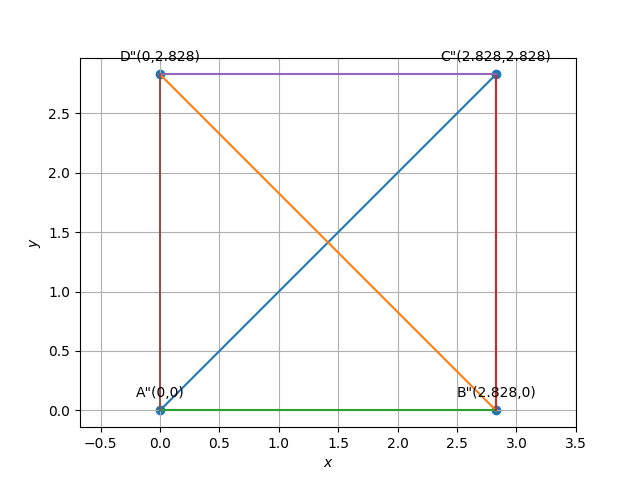
\includegraphics[width=\columnwidth]{chapters/10/7/4/4/figs/square2}
	\end{center}
\caption{}
\label{fig:7/4/4/4Fig3}
\end{figure}

\newpage
\iffalse
Again tranforming(rotating) the coordinates back to the original axis.

We know for anti-clockwise direction the rotation matrix is given as
\begin{align}
\vec{P} =
\myvec{
\cos\theta & -\sin\theta \\
\sin\theta & \cos\theta \\
}
\end{align}

Again we know that the angle is negative so the rotation will be in clockwise direction. So now the transformed(rotated) coordinates $\vec{B} \text{ and } \vec{D}$ are with refrence to 
\fi
from Figure 
%\ref{fig:7/4/4/4Fig4},
\ref{fig:7/4/4/4Fig3},
\begin{align}
	\vec{C^{\prime \prime}} &= \vec{P} (\vec{C}-\vec{A}) 
	\\
\label{eq:7/4/4/4bp}
	\vec{B^{\prime \prime}} &= \myvec{\vec{e}_1 & \vec{0}}\vec{C^{\prime \prime}}
	\\
\label{eq:7/4/4/4dp}
	\vec{D^{\prime \prime}} &= \myvec{ \vec{0} & \vec{e}_2}\vec{C^{\prime \prime}}
\end{align}
Now, 
\begin{align}
\label{eq:7/4/4/4b}
	\vec{B} = \vec{P}^{\top}\vec{B}^{\prime \prime}+\vec{A}
	\\
\label{eq:7/4/4/4d}
	\vec{D} = \vec{P}^{\top}\vec{D}^{\prime \prime}+\vec{A}
\end{align}
by reversing the process of translation and rotation.  Thus, 
from
\eqref{eq:7/4/4/4b}
\eqref{eq:7/4/4/4bp},
\eqref{eq:7/4/4/4d}
and
\eqref{eq:7/4/4/4dp}
\begin{align}
	\vec{B} = \vec{P}^{\top}\myvec{\vec{e}_1 & \vec{0}}\vec{P} (\vec{C}-\vec{A}) +\vec{A}
	\\
	\vec{D} = \vec{P}^{\top}\myvec{\vec{0} & \vec{e}_2  }\vec{P} (\vec{C}-\vec{A}) +\vec{A}
%	\vec{B} &= \brak{(\vec{C}-\vec{A})^{\top}\vec{P}^{\top} \vec{e}_1}\vec{P}^{\top}\vec{e}_1+\vec{A}
%	\\
%	\vec{D} &= \brak{(\vec{C}-\vec{A})^{\top}\vec{P}^{\top} \vec{e}_2}\vec{P}^{\top}\vec{e}_2+\vec{A}
\end{align}
yielding
		\begin{align}
\vec{B}=
\myvec{
1\\
0
},
\vec{D}
\myvec{
1\\
4
}.
		\end{align}
\iffalse
\begin{align}
\vec{B^{\prime}} &= \vec{P}\vec{B^{\prime \prime}} = \myvec{
\frac{1}{\sqrt{2}} & \frac{1}{\sqrt{2}} \\
-\frac{1}{\sqrt{2}} & \frac{1}{\sqrt{2}}\\
}
\myvec{
 \frac{4}{\sqrt{2}}\\
 0\\
} = 
\myvec{
2 \\
-2\\
}\\
\vec{D^{\prime}} &= \vec{P}\vec{D^{\prime \prime}} = \myvec{
\frac{1}{\sqrt{2}} & \frac{1}{\sqrt{2}} \\
-\frac{1}{\sqrt{2}} & \frac{1}{\sqrt{2}}\\
}
\myvec{
 0\\
 \frac{4}{\sqrt{2}}\\
} = 
\myvec{
2 \\
2 \\
}
\end{align}

\begin{figure}[!h]
	\begin{center} 
	    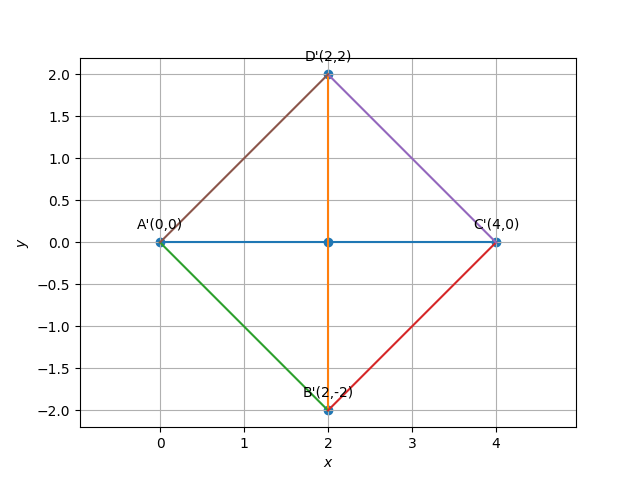
\includegraphics[width=\columnwidth]{chapters/10/7/4/4/figs/square3}
	\end{center}
\caption{}
\label{fig:7/4/4/4Fig4}
\end{figure}

Again transforming(shifting) the axis back to the original with refrence to Figure \ref{fig:7/4/4/4Fig5}
\begin{align}
\vec{B} &= \vec{B^{\prime}}+\vec{A} = \myvec{
2 \\
-2\\
}+\myvec{
-1 \\
2\\
} = 
\myvec{
1 \\
0\\
}\\
\vec{D} &= \vec{D^{\prime}}+\vec{A} = \myvec{
2 \\
2\\
}+\myvec{
-1 \\
2\\
} = 
\myvec{
1 \\
4 \\
}
\end{align}

Hence, the other two vertices are $\vec{B}(1,0) \text{ and } \vec{D}(1,4)$   

\begin{figure}[!h]
	\begin{center} 
	    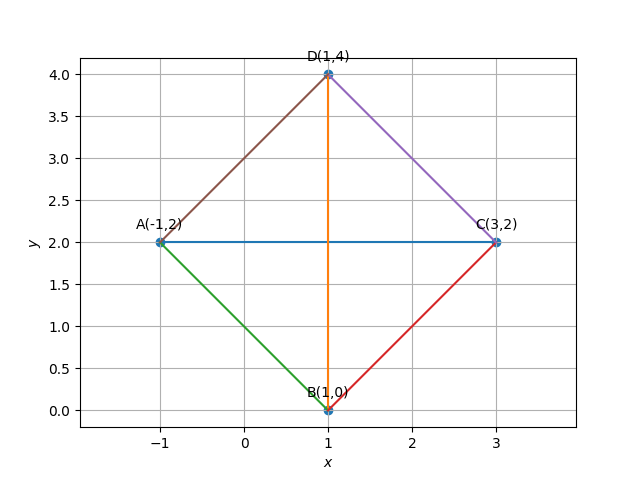
\includegraphics[width=\columnwidth]{chapters/10/7/4/4/figs/square4}
	\end{center}
\caption{}
\label{fig:7/4/4/4Fig5}
\end{figure}
which can also be expressed as
\begin{align}
\vec{B} &= \vec{A} + \vec{P}\myvec{
\vec{e_{1}}&\vec{0}\\
}
\vec{P}^\top \brak{\vec{C}-\vec{A}}\\
\vec{D} &= \vec{A} + \vec{P}\myvec{
\vec{0}&\vec{e_{2}}\\
}
\vec{P}^\top \brak{\vec{C}-\vec{A}}\\
\end{align}
where $\vec{P}$ is the rotation matrix and $\vec{A} \text{ and } \vec{C}$ are the position vectors of opposite vertices.

Derivation of the above formulas:

We know that after shifting the axis and rotating by the required angle any arbitrary square will be aligned with the x and y axis so that we can directly get the vectors $\vec{B} \text{ and } \vec{D}$ as follows
\begin{align}
\vec{C^{\prime\prime}} &= \vec{P}^\top \brak{\vec{C} - \vec{A}}\\
\vec{B^{\prime\prime}} &= \myvec{
\vec{e_{1}} & \vec{0}
}\vec{C^{\prime\prime}} = \myvec{
\vec{e_{1}} & \vec{0}
}\vec{P}^\top \brak{\vec{C} - \vec{A}}\\
\vec{B^{\prime}} &= \vec{P} \vec{B^{\prime\prime}}  = \vec{P}\myvec{
\vec{e_{1}} & \vec{0}
}\vec{P}^\top \brak{\vec{C} - \vec{A}}\\
\vec{B} &= \vec{A}+\vec{B^{\prime}}\\
 &= \vec{A} + \vec{P}\myvec{
\vec{e_{1}}&\vec{0}\\
}
\vec{P}^\top\brak{\vec{C}-\vec{A}}
\end{align}

Similarly for D it can be derived as
\begin{align}
\vec{C^{\prime\prime}} &= \vec{P}^\top \brak{\vec{C} - \vec{A}}\\
\vec{D^{\prime\prime}} &= \myvec{
\vec{0} & \vec{e_{2}}
}\vec{C^{\prime\prime}} = \myvec{
\vec{0} & \vec{e_{2}}
}\vec{P}^\top \brak{\vec{C} - \vec{A}}\\
\vec{D^{\prime}} &= \vec{P} \vec{D^{\prime\prime}} = \vec{P} \myvec{
\vec{0} & \vec{e_{2}}
}\vec{P}^\top \brak{\vec{C} - \vec{A}}\\
\vec{D} &= \vec{A}+\vec{D^{\prime}}\\
 &= \vec{A} + \vec{P}\myvec{
\vec{0}&\vec{e_{2}}\\
}
\vec{P}^\top\brak{\vec{C}-\vec{A}}
\end{align}


Verification of the above formula for the given question

\begin{align}
\vec{B} &= \myvec{
-1\\
2\\
}+\myvec{
\frac{1}{\sqrt{2}} & \frac{1}{\sqrt{2}} \\
-\frac{1}{\sqrt{2}} & \frac{1}{\sqrt{2}}\\
}\myvec{
 1&0\\
 0&0\\
}\myvec{
\frac{1}{\sqrt{2}} & -\frac{1}{\sqrt{2}} \\
\frac{1}{\sqrt{2}} & \frac{1}{\sqrt{2}}\\
}\myvec{
4\\
0\\
}\\
 &= \myvec{
-1\\
2\\
}+\myvec{
\frac{1}{\sqrt{2}} & \frac{1}{\sqrt{2}} \\
-\frac{1}{\sqrt{2}} & \frac{1}{\sqrt{2}}\\
}\myvec{
 1&0\\
 0&0\\
}\myvec{
\frac{4}{\sqrt{2}}\\
\frac{4}{\sqrt{2}}\\
}\\
 &= \myvec{
-1\\
2\\
}+\myvec{
\frac{1}{\sqrt{2}} & \frac{1}{\sqrt{2}} \\
-\frac{1}{\sqrt{2}} & \frac{1}{\sqrt{2}}\\
}\myvec{
\frac{4}{\sqrt{2}}\\
0\\
}\\
 &= \myvec{
-1\\
2\\
}+\myvec{
2\\
-2\\
}\\
 &= \myvec{
1\\
0\\
}\\
\vec{D} &= \myvec{
-1\\
2\\
}+\myvec{
\frac{1}{\sqrt{2}} & \frac{1}{\sqrt{2}} \\
-\frac{1}{\sqrt{2}} & \frac{1}{\sqrt{2}}\\
}\myvec{
 0&0\\
 0&1\\
}\myvec{
\frac{1}{\sqrt{2}} & -\frac{1}{\sqrt{2}} \\
\frac{1}{\sqrt{2}} & \frac{1}{\sqrt{2}}\\
}\myvec{
4\\
0\\
}\\
 &= \myvec{
-1\\
2\\
}+\myvec{
\frac{1}{\sqrt{2}} & \frac{1}{\sqrt{2}} \\
-\frac{1}{\sqrt{2}} & \frac{1}{\sqrt{2}}\\
}\myvec{
 0&0\\
 0&1\\
}\myvec{
\frac{4}{\sqrt{2}}\\
\frac{4}{\sqrt{2}}\\
}\\
 &= \myvec{
-1\\
2\\
}+\myvec{
\frac{1}{\sqrt{2}} & \frac{1}{\sqrt{2}} \\
-\frac{1}{\sqrt{2}} & \frac{1}{\sqrt{2}}\\
}\myvec{
0\\
\frac{4}{\sqrt{2}}\\
}\\
 &= \myvec{
-1\\
2\\
}+\myvec{
2\\
2\\
}\\
 &= \myvec{
1\\
4\\
}
\end{align}
\fi








\item The base of an equilateral triangle with side $2a$ lies along the y-axis such that the mid-point of the base is at the origin. Find vertices of the triangle.
\label{chapters/11/10/1/2}
\iffalse
\documentclass[journal,12pt,twocolumn]{IEEEtran}
\usepackage{graphicx}
\usepackage{listings}
\usepackage[utf8]{inputenc}
\usepackage{caption}
\usepackage{hyperref}
\usepackage[cmex10]{amsmath}
\usepackage{array}
\usepackage{gensymb}
\usepackage{booktabs}
\usepackage{etoolbox}
\patchcmd{\section}{\centering}{}{}{}
\providecommand{\norm}[1]{\left\lVert#1\right\rVert}
\providecommand{\abs}[1]{\left\vert#1\right\vert}
\let\vec\mathbf
\newcommand{\myvec}[1]{\ensuremath{\begin{pmatrix}#1\end{pmatrix}}}
\newcommand{\mydet}[1]{\ensuremath{\begin{vmatrix}#1\end{vmatrix}}}
\providecommand{\brak}[1]{\ensuremath{\left(#1\right)}}
\makeatletter
\newcommand\xleftrightarrow[2][]{%
  \ext@arrow 9999{\longleftrightarrowfill@}{#1}{#2}}
\newcommand\longleftrightarrowfill@{%
  \arrowfill@\leftarrow\relbar\rightarrow}
\makeatother
\title{Matrix Problems \textbf{\\Straight Lines }}
\author{Manoj Chavva} 

\begin{document}
\maketitle



\section{Problem Statement}

\noindent 
\fi
	\begin{figure}[!ht]
		\centering
 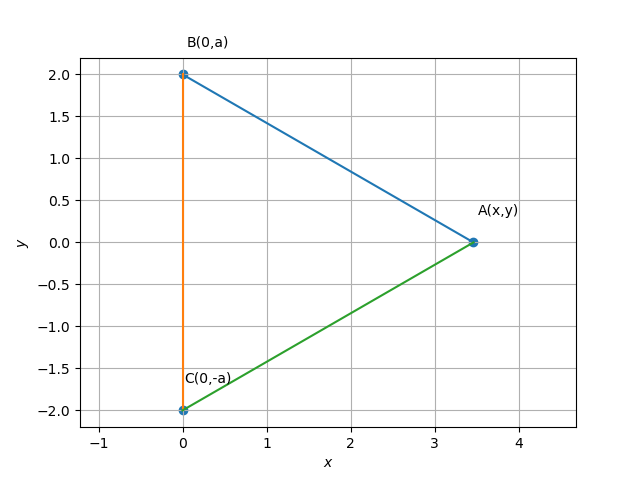
\includegraphics[width=\columnwidth]{chapters/11/10/1/2/figs/triangle.png}
		\caption{}
		\label{fig:11/10/1/2}
  	\end{figure}
	\\
	\solution Let the base be $BC$.  From the given information, 
\begin{align}
	\vec{B} = a\vec{e}_2,
	\vec{C} = -a\vec{e}_2
\end{align}
Since $\vec{A}$ lies on the $x$-axis, 
\begin{align}
	\vec{A} = k\vec{e}_1
\end{align}
and 
\begin{align}
	\norm{\vec{A}-\vec{C}}^2 &= \brak{2a}^2
	\\
	\implies \norm{\vec{A}}^2+\norm{\vec{C}}^2 - 2 \vec{A}^{\top}\vec{C} &= 4a^2
	\\
	\implies k^2 +a^2 &= 4a^2
	\\
	\text{or, } k = \pm a\sqrt{3}
\end{align}
Thus, 
\begin{align}
	\vec{A} = \pm \sqrt{3}a\vec{e}_1
\end{align}
		Fig. \ref{fig:11/10/1/2}
		is plotted for $a = 2$.

\iffalse

\begin{figure}[h]
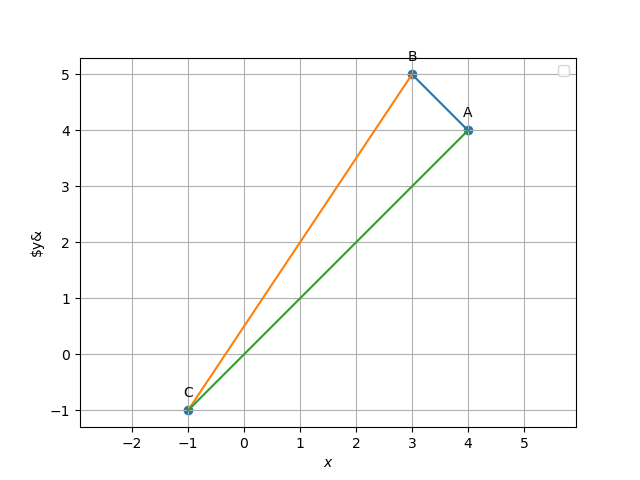
\includegraphics[width=1\columnwidth]{triangle.png}
\caption{Equilateral Triangle ABC}
\label{fig:triangle}
\end{figure}

\section{Construction}
B and C are the inputs.
\begin{table}[h]
\centering
\large
\begin{tabular}{|l|l|l|}
\hline
\textbf{Symbol} & \textbf{Value} & \textbf{Description} \\ \hline
B               & \myvec{0 \\ 2}         & Vertex B             \\ \hline
C               & \myvec{0 \\ -2}        & Vertex C             \\ \hline
A               & \myvec{x \\ y}          & Vertex A             \\ \hline
A1              & \myvec{x1 \\ y1}       & Vertex A             \\ \hline
\end{tabular}
\end{table}

\section{Solution}
\noindent Given the base with 2a is lies on the y-axis with the mid-point of the base is at origin. The vertices of the two points on y-axis will be

\begin{equation}
\vec{B}=\begin{pmatrix} 
0\\
a
\end{pmatrix}, {
\vec{C}=\begin{pmatrix} 
0\\
-a
\end{pmatrix} }
\end{equation}
\noindent Given $\Delta$ABC is an equilateral triangle i.e 
\begin{equation}
 \norm{\vec{A}-\vec{B}}= \norm{\vec{B}-\vec{C}}= \norm{\vec{C}-\vec{A}} =2a
\end{equation}

%\noindent As AB = AC, triangle is isoceles and by properties of isoceles triangle, altitude is perpendicular bisector of base.\\
%
%\noindent Therefore $\angle$AOC = $\angle$AOB = $90^0$ and $\norm{\vec{O}-\vec{B}}= \norm{\vec{O}-\vec{C}}= a$ \\
%
%\noindent By Cosine laws,
%\begin{equation}
%\cos\vec{B} = \cos\vec{C} = a* \frac{1}{2a} = \frac{1}{2}
%\end{equation}
%\begin{equation}
%\angle B = \angle C = \arccos\frac{1}{2} = 60^0
%\end{equation}
% \begin{equation}
% \angle A = 180^0 -(60^0 * 2) = 60^0
%  \end{equation}
%\noindent Therefore, the equilaterial triangle have all internal angles eaqual to  $60^0$ 

\noindent Consider, two sides of equilateral triangle be $\vec{A}$ and $\vec{B}$ then the third side will be $ \vec{A} -\vec{B}$ 
%Hence,
%\begin{equation}
%\norm{\vec{a}-\vec{b}}^2 = l
%\end{equation}
%\begin{equation}
%\brak{\vec{a}-\vec{b}}^{\top} \brak{\vec{a}-\vec{b}} = l^2
%\end{equation}
%\begin{equation}
%l^2 = 2 \vec{a}^{\top} \cdot \vec{b}
%\end{equation}
%\begin{equation}
%l^2 = 2 \norm{\vec{a}}\norm{\vec{b}} \cos\theta
%\end{equation}
%\begin{equation}
%\theta = \arccos\frac{1}{2} = 60^0
\begin{equation}
\norm{\vec{A}}=\norm{\vec{B}}=\norm{\vec{A-B}}\\
\end{equation}
\begin{equation}
\norm{\vec{A}}^2=\norm{\vec{B}}^2=\norm{\vec{A-B}}^2\\
\end{equation}
\begin{equation}
\norm{\vec{A}}^2+\norm{\vec{B}}^2-2\vec{A}^T\vec{B}=\norm{\vec{A}}^2=\norm{\vec{B}}^2\\
\end{equation}
\begin{equation}
\frac{\vec{A}^T\vec{B}}{\norm{\vec{A}}^2}=\frac{\vec{A}^T\vec{B}}{\norm{\vec{B}^2}}=\frac{1}{2}
\end{equation}
%$\triangle$OAB is a equilateral triangle\\

\noindent Therefore, the  triangle have all internal angles eaqual to  $60^0$

The angle between two vectors is given by 
  \begin{align}
    \label{eq:angle2d}
    \theta = \cos^{-1}\frac{\vec{A}^{\top} \vec{B}}{\norm{A}\norm{B}}
  \end{align}

 \begin{equation}  
  \brak{\vec{x}-\vec{B}}^{\top} \brak{\vec{x}-\vec{C}}= \norm{\vec{x}-\vec{B}} \cdot \norm{\vec{x}-\vec{C}} \cdot \cos\theta 
 \end{equation}

 \begin{equation}  
\brak{\vec{x}^\top \cdot \vec{x}} - \brak{\vec{x}^\top \cdot \vec{C}} - \brak{\vec{B}^\top \cdot \vec{x}} - \brak{\vec{B}^\top \cdot \vec{C}} = 2a \cdot 2a \cos 60^0   
 \end{equation}

 \begin{equation}  
\norm{\vec{x}}^2 - \vec{x}^\top\brak{\vec{B}+\vec{C}} - \vec{B}^\top \cdot \vec{C} = 2a \cdot 2a \cdot \frac{1}{2}
 \end{equation}

  \begin{equation}  
\norm{\vec{x}}^2 - \vec{x}^\top\brak{0} -\myvec{0 \\ a} \myvec{0 & -a}  = 4a^2
 \end{equation}

\begin{equation}
\norm{\vec{x}}^2 + a^2 = 4a^2
\end{equation}

\begin{equation}
\norm{\vec{x}}^2 = 3a^2
\label{eq-1}
\end{equation}
Considering, the line equation of $\vec{AB}$

\begin{equation}
\norm{\vec{x}-\vec{B}}^2 = 4a^2
\end{equation}

\begin{equation}
\brak{\vec{x} -\vec{B}}^{\top} \cdot \brak{\vec{x}-\vec{B}} = 4a^2
\end{equation}

\begin{equation}
\norm{\vec{x}}^2-2\cdot \vec{x}^\top \vec{B} + \norm{\vec{B}}^2 = 4a^2
\end{equation}

\begin{equation}
3a^2 - 2\cdot \vec{x}^\top \vec{B} + a^2 = 4a^2
\end{equation}

\begin{equation}
\vec{x}^\top \vec{B} = 0
\end{equation}
\noindent Since we can write, \begin{equation}
\vec{B} = a \cdot \vec{e}_2
\end{equation}

\begin{equation}
\vec{x}^\top \cdot a \cdot \vec{e}_2 = 0
\end{equation}

\begin{equation}
\vec{x}^\top \cdot \vec{e}_2 = 0
\end{equation}

\begin{equation}
\vec{x} = \lambda \vec{e}_1
\end{equation}

\noindent From this its clearly concluded that third vertex will lie on x-axis. 
\noindent From the equation \eqref{eq-1} 
\begin{equation}
\vec{x} = \sqrt{3}{a}
\end{equation}


\noindent Hence,the coordinates of the vertices of triangle are 
  \begin{equation*}
\vec{A} = 
   \begin{pmatrix}
   \pm\sqrt{3}a \\ 0
 \end{pmatrix}
 \end{equation*}

\begin{equation}
\vec{B}=\begin{pmatrix} 
0\\
a
\end{pmatrix}, {
\vec{C}=\begin{pmatrix} 
0\\
-a
\end{pmatrix} }
\end{equation}



\begin{table}[h]
\large
\begin{tabular}{lll}
\multicolumn{3}{l}{Get Python Code for image from}                                                 \\ \hline
\multicolumn{3}{|l|}{\url{https://github.com/ManojChavva/FWC/blob/main/Matrix/line/code-py/triangle.py}} \\ 
 \hline
\multicolumn{3}{l}{Get LaTex code from}                                                            \\ \hline
\multicolumn{3}{|l|}{\url{https://github.com/ManojChavva/FWC/blob/main/Matrix/line/line.tex}}            \\ \hline
\end{tabular}
\end{table}

\end{document}

\fi

\item Without using distance formula, show that points (– 2, – 1), (4, 0), (3, 3) and (–3, 2) are the vertices of a parallelogram.
\label{chapters/11/10/1/9}

\iffalse
\documentclass[A4,12pt,twocolumn]{IEEEtran}
%
\usepackage{setspace}
\usepackage{gensymb}
%\doublespacing
\singlespacing

%\usepackage{graphicx}
%\usepackage{amssymb}
%\usepackage{relsize}
\usepackage[cmex10]{amsmath}
%\usepackage{amsthm}
%\interdisplaylinepenalty=2500
%\savesymbol{iint}
%\usepackage{txfonts}
%\restoresymbol{TXF}{iint}
%\usepackage{wasysym}
\usepackage{amsthm}
%\usepackage{iithtlc}
\usepackage{mathrsfs}
\usepackage{txfonts}
\usepackage{stfloats}
\usepackage{bm}
\usepackage{cite}
\usepackage{cases}
\usepackage{subfig}
%\usepackage{xtab}
\usepackage{longtable}
\usepackage{multirow}
%\usepackage{algorithm}
%\usepackage{algpseudocode}
\usepackage{enumitem}
\usepackage{mathtools}
\usepackage{steinmetz}
\usepackage{tikz}
\usepackage{circuitikz}
\usepackage{verbatim}
\usepackage{tfrupee}
\usepackage[breaklinks=true]{hyperref}
%\usepackage{stmaryrd}
\usepackage{tkz-euclide} % loads  TikZ and tkz-base
%\usetkzobj{all}
\usetikzlibrary{calc,math}
\usepackage{listings}
    \usepackage{color}                                            %%
    \usepackage{array}                                            %%
    \usepackage{longtable}                                        %%
    \usepackage{calc}                                             %%
    \usepackage{multirow}                                         %%
    \usepackage{hhline}                                           %%
    \usepackage{ifthen}                                           %%
  %optionally (for landscape tables embedded in another document): %%
    \usepackage{lscape}     
\usepackage{multicol}
\usepackage{chngcntr}
%\usepackage{enumerate}

%\usepackage{wasysym}
%\newcounter{MYtempeqncnt}
\DeclareMathOperator*{\Res}{Res}
%\renewcommand{\baselinestretch}{2}
\renewcommand\thesection{\arabic{section}}
\renewcommand\thesubsection{\thesection.\arabic{subsection}}
\renewcommand\thesubsubsection{\thesubsection.\arabic{subsubsection}}

\renewcommand\thesectiondis{\arabic{section}}
\renewcommand\thesubsectiondis{\thesectiondis.\arabic{subsection}}
\renewcommand\thesubsubsectiondis{\thesubsectiondis.\arabic{subsubsection}}

% correct bad hyphenation here
\hyphenation{op-tical net-works semi-conduc-tor}
\def\inputGnumericTable{}                                 %%

\lstset{
%language=C,
frame=single, 
breaklines=true,
columns=fullflexible
}
%\lstset{
%language=tex,
%frame=single, 
%breaklines=true
%}

\begin{document}
%


\newtheorem{theorem}{Theorem}[section]
\newtheorem{problem}{Problem}
\newtheorem{proposition}{Proposition}[section]
\newtheorem{lemma}{Lemma}[section]
\newtheorem{corollary}[theorem]{Corollary}
\newtheorem{example}{Example}[section]
\newtheorem{definition}[problem]{Definition}
%\newtheorem{thm}{Theorem}[section] 
%\newtheorem{defn}[thm]{Definition}
%\newtheorem{algorithm}{Algorithm}[section]
%\newtheorem{cor}{Corollary}
\newcommand{\BEQA}{\begin{eqnarray}}
\newcommand{\EEQA}{\end{eqnarray}}
\newcommand{\define}{\stackrel{\triangle}{=}}

\bibliographystyle{IEEEtran}
%\bibliographystyle{ieeetr}


\providecommand{\mbf}{\mathbf}
\providecommand{\pr}[1]{\ensuremath{\Pr\left(#1\right)}}
\providecommand{\qfunc}[1]{\ensuremath{Q\left(#1\right)}}
\providecommand{\sbrak}[1]{\ensuremath{{}\left[#1\right]}}
\providecommand{\lsbrak}[1]{\ensuremath{{}\left[#1\right.}}
\providecommand{\rsbrak}[1]{\ensuremath{{}\left.#1\right]}}
\providecommand{\brak}[1]{\ensuremath{\left(#1\right)}}
\providecommand{\lbrak}[1]{\ensuremath{\left(#1\right.}}
\providecommand{\rbrak}[1]{\ensuremath{\left.#1\right)}}
\providecommand{\cbrak}[1]{\ensuremath{\left\{#1\right\}}}
\providecommand{\lcbrak}[1]{\ensuremath{\left\{#1\right.}}
\providecommand{\rcbrak}[1]{\ensuremath{\left.#1\right\}}}
\theoremstyle{remark}
\newtheorem{rem}{Remark}
\newcommand{\sgn}{\mathop{\mathrm{sgn}}}
\providecommand{\abs}[1]{\left\vert#1\right\vert}
\providecommand{\res}[1]{\Res\displaylimits_{#1}} 
\providecommand{\norm}[1]{\left\lVert#1\right\rVert}
%\providecommand{\norm}[1]{\lVert#1\rVert}
\providecommand{\mtx}[1]{\mathbf{#1}}
\providecommand{\mean}[1]{E\left[ #1 \right]}
\providecommand{\fourier}{\overset{\mathcal{F}}{ \rightleftharpoons}}
%\providecommand{\hilbert}{\overset{\mathcal{H}}{ \rightleftharpoons}}
\providecommand{\system}{\overset{\mathcal{H}}{ \longleftrightarrow}}
	%\newcommand{\solution}[2]{\textbf{Solution:}{#1}}
\newcommand{\solution}{\noindent \textbf{Solution: }}
\newcommand{\cosec}{\,\text{cosec}\,}
\providecommand{\dec}[2]{\ensuremath{\overset{#1}{\underset{#2}{\gtrless}}}}
\newcommand{\myvec}[1]{\ensuremath{\begin{pmatrix}#1\end{pmatrix}}}
\newcommand{\mydet}[1]{\ensuremath{\begin{vmatrix}#1\end{vmatrix}}}
%\numberwithin{equation}{section}
\numberwithin{equation}{subsection}
%\numberwithin{problem}{section}
%\numberwithin{definition}{section}
\makeatletter
\@addtoreset{figure}{problem}
\makeatother

\let\StandardTheFigure\thefigure
\let\vec\mathbf
%\renewcommand{\thefigure}{\theproblem.\arabic{figure}}
\renewcommand{\thefigure}{\theproblem}
%\setlist[enumerate,1]{before=\renewcommand\theequation{\theenumi.\arabic{equation}}
%\counterwithin{equation}{enumi}


%\renewcommand{\theequation}{\arabic{subsection}.\arabic{equation}}

\def\putbox#1#2#3{\makebox[0in][l]{\makebox[#1][l]{}\raisebox{\baselineskip}[0in][0in]{\raisebox{#2}[0in][0in]{#3}}}}
     \def\rightbox#1{\makebox[0in][r]{#1}}
     \def\centbox#1{\makebox[0in]{#1}}
     \def\topbox#1{\raisebox{-\baselineskip}[0in][0in]{#1}}
     \def\midbox#1{\raisebox{-0.5\baselineskip}[0in][0in]{#1}}

\vspace{3cm}


\title{QUIZ 4}
\author{Shristy Sharma (EE22BNITS11001)}





% make the title area
\maketitle

\newpage

%\tableofcontents

\bigskip

\renewcommand{\thefigure}{\theenumi}
\renewcommand{\thetable}{\theenumi}
%\renewcommand{\theequation}{\theenumi}


%Download all python codes 
%
%\begin{lstlisting}
%svn co https://github.com/JayatiD93/trunk/My_solution_design/codes
%\end{lstlisting}

%Download all and latex-tikz codes from 
%
%\begin{lstlisting}
%svn co https://github.com/gadepall/school/trunk/ncert/geometry/figs
%\end{lstlisting}
%


\section{PROBLEM 1}
1. Without using distance formula, show that points $\vec{A}$ = $\myvec{ -2\\-1}$,\ $\vec{B}$ = $\myvec{ 4\\0}$ ,\ $\vec{C}$ = $\myvec{ 3\\3}$ and \ $\vec{D}$ = $\myvec{ -3\\2}$ \
are the vertices of a parallelogram.\\
\\SOLUTION:\\
Given,
\begin{align}
\vec{A} = \myvec{ -2\\-1} , \vec{B} = \myvec{ 4\\0}, \vec{C} = \myvec{3\\3} , \vec{D} =\myvec{-3\\2} 
\end{align}
\fi
To show that the given points are the vertices of a parallelogram, we need to show the following
\begin{enumerate}
\item $\vec{A}-\vec{B} = \vec{D}-\vec{C} $
\item  $\vec{A}-\vec{D} = \vec{B}-\vec{C} $
 \end{enumerate}
So,
\begin{align}
\vec{A}-\vec{B} &= \myvec{-2\\-1} - \myvec{4\\0}\\ &= \myvec{-6\\-1}\\
\vec{D}-\vec{C} &= \myvec{-3\\2} - \myvec{3\\3}\\ &= \myvec{-6\\-1}\\
\vec{A}-\vec{D} &= \myvec{-2\\-1} - \myvec{-3\\2}\\ &= \myvec{1\\-3}\\
\vec{B}-\vec{C} &= \myvec{4\\0} - \myvec{ 3\\3}\\ &= \myvec{1\\-3}
\end{align}
Therefore, we can now say that the given points are the vertices of a parallelogram since both the sides of the quadrilateral are parallel to each other.
See Fig.      \ref{fig:chapters/11/10/1/91}.
\begin{figure}[h!]
  \centering
   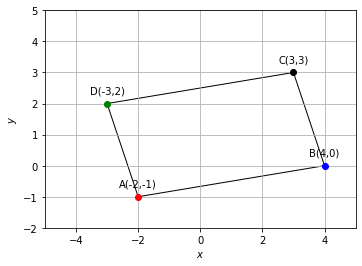
\includegraphics[width=\columnwidth]{chapters/11/10/1/9/figs/paralellogram.png}
    \caption{}
     \label{fig:chapters/11/10/1/91}  
\end{figure}




\item A line passes through $(x_1,y_1)$ and $(h,k)$. If slope of the line is m show that $(k-y_1)=m(h-x_1)$.
\label{chapters/11/10/1/12}
\iffalse 
\documentclass[journal,12pt,twocolumn]{IEEEtran}
\usepackage{graphicx}
\graphicspath{{./figs/}}{}
\usepackage{amsmath,amssymb,amsfonts,amsthm}
\newcommand{\myvec}[1]{\ensuremath{\begin{pmatrix}#1\end{pmatrix}}}

\let\vec\mathbf

\title{
Matrix-Lines
}
\author{R.Radhika}
\begin{document}
\maketitle
\tableofcontents
\bigskip
\section{Problem Statement}
\fi
\\
\solution 
	\begin{figure}[!ht]
		\centering
 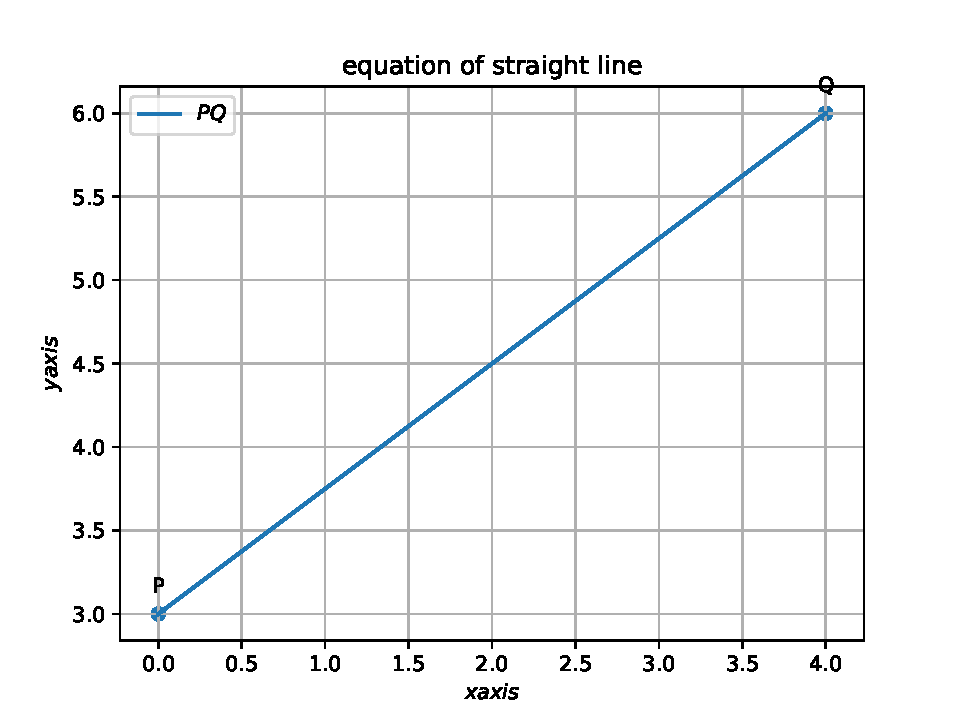
\includegraphics[width=\columnwidth]{chapters/11/10/1/12/figs/figure.pdf}
		\caption{}
		\label{fig:11/10/1/12}
  	\end{figure}
\iffalse
\section{Construction}
\begin{figure}[h]
    \centering
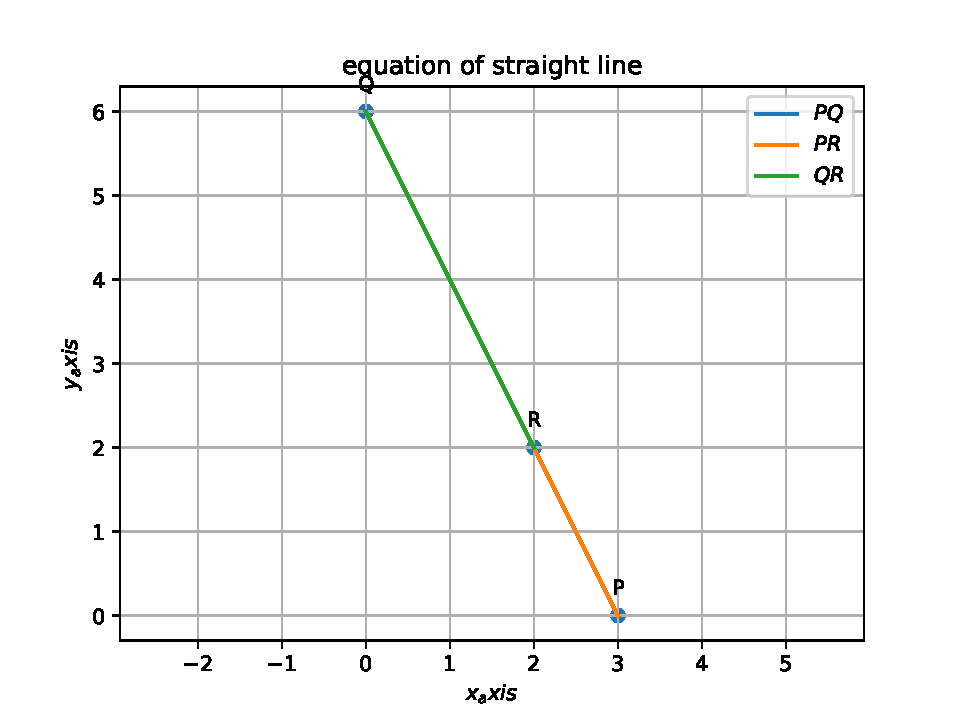
\includegraphics[width=\columnwidth]{figure.pdf}
    \caption{Equation of the slope}
    \label{fig:my_label}
\end{figure}
\vspace{2cm}
\begin{table}[h]
    \centering
    \begin{tabular}{|c|c|c|}
       \hline
       \textbf{Symbol}&\textbf{Value}&\textbf{Description}  \\
       \hline
	    $\vec{A}$ & $\myvec{
		    x_1\\
		    y_1}$
	    & Point on X-axis\\
        \hline
	    $\vec{B}$ & $\myvec{h\\k}$
 & Point on Y-axis\\
        \hline
        \hline
        A & k-y1=m(h-x1) & Given Condition\\
        \hline
    \end{tabular}
    \caption{Parameters}
    \label{tab:my_label}
\end{table}


\section{Solution}
Given that resultant line passes through point(x1,y1) and (h,k) (let prove the equation in vector form by line eqation ) \\
\\
\\
\fi
Given 
\begin{align}
\vec{A}=\myvec{
  x_1\\
  y_1}
 , \vec{B}=\myvec{
  h\\
  k}
\end{align}

\iffalse
\textbf{First Method}:\\
condition is	
\begin{equation}
	{\vec{n^{\top}}\vec{{m}}} = 0 \\     \label{eq-1}
\end{equation}	
m is 
\fi
The direction vector
\begin{align}
	\vec{m} &= \vec{B}-\vec{A}
	\\
	&=
	\myvec{
  h-x_1\\
  k-y_1
  }
   \equiv
	\myvec{
1\\
	\frac{ k-y_1}{h-x_1}
  }
\end{align}
which yields the desired relation from 
		\eqref{eq:two-dir-vec}.
\iffalse
\begin{equation}
 			\myvec{
					-m& 1}\myvec{
  h-x_1\\
  k-y_1
  }
   = 0  \label{eq-4}
\end{equation}
by solving eq-4
\begin{equation}
	\myvec{
 -m (h-x_1))+(k-y_1}=0
\end{equation}
Then the equation becomes\\

$\myvec{
  k-y_1)=m(h-x_1}$\\
Therefore the Resultant Equation of line is\\
\begin{equation}
	\myvec{
  k-y_1)=m(h-x_1}
\end{equation}
\begin{table}[h]
    \centering
    \begin{tabular}{|c|}
    \hline \\
           \myvec{
  k-y_1)=m(h-x_1}\\
         \\
\hline
    \end{tabular}
\end{table}\\
\textbf{Second Method}:\\
given ${\vec{A}}$=$\myvec{
  x_1\\
  y_1}$
  ${\vec{B}}$=$\myvec{
  h\\
  k}$\\
C=$\myvec{
  \frac{x_1+h}{2}\\
  \frac{y_1+k}{2}
}$\\
m is the direction vector\\

		 m=C-A\\
		 
		 m=B-C\\
		 		 
m=$\myvec{
  \frac{x_1+h}{2}-x_1\\
  \frac{y_1+k}{2}-y_1
}$\\

 m=2$\myvec{
  \frac{h-x_1}{2}\\
  \frac{k-y_1}{2}
}$\\

m=$\myvec{
  {h-x_1}\\
  {k-y_1}
}$\\

condition is	
\begin{equation}
	{\vec{n^{\top}}\vec{{m}}} = 0 \\     \label{eq-1}
\end{equation}
\begin{equation}
 			\myvec{
					-m& 1}\myvec{
  h-x_1\\
  k-y_1
  }
   = 0  \label{eq-4}
\end{equation}
by solving eq-4
\begin{equation}
	\myvec{
 -m (h-x_1))+(k-y_1}=0
\end{equation}
Then the equation becomes\\

$\myvec{
  k-y_1)=m(h-x_1}$\\
Therefore the Resultant Equation of line is\\
\begin{equation}
	\myvec{
  k-y_1)=m(h-x_1}
\end{equation}			 


\textbf{Third Method}:\\
\begin{equation}
	{\vec{n^{\top}}\vec{{m}}} = 0 \\     \label{eq-1}
\end{equation}		
\begin{equation}
	{\vec{n^{\top}}\vec{({x}-A)}} = 0 \\     \label{eq-2}
\end{equation}
\begin{equation}
	{\vec{n^{\top}}\vec{({x}-B)}} = 0      \label{eq-3}
\end{equation}


 The Equation of line through ${\vec{A}}$  from 1 is\\
\begin{equation}
	\vec{n^{\top}}\myvec{ 
	\myvec{
  x\\
  y}
  - \label{eq-4}
	\myvec{
  x_1\\
  y_1}}
   = 0 \
\end{equation}
\\
Equation of line passing through ${\vec{B}}$ from 2 is\\
\begin{equation}
	\vec{n^{\top}}\myvec{ 
	\myvec{
  x\\
  y}
  - \label{eq-5}
	\myvec{
  h\\
  k}}
  = 0 \
\end{equation}
\\
Now by solving eq3,\\
\begin{equation}
	\vec{n^{\top}}
	\myvec{
  x-x_1\\
  y-y_1
}
  = 0 \label{eq-6}
\end{equation}
 
Now by solving eq4,\\
\begin{equation}
	\vec{n^{\top}}
	\myvec{
  x-h\\
  y-k
}
  = 0 \label{eq-7}
\end{equation}
 \\
 From eq5 and eq6 we can prove the equation ${\vec{n}}$,\\
 \\
 \begin{equation}
 			\myvec{
					-m& 1}\myvec{
  x-x_1& y-y_1\\
  x-h & y-k
 }
	 = 0   \
\end{equation}\\
 by solving 7 th equation\\
 \begin{equation}
	\myvec{
  k-y_1)=m(h-x_1}
\end{equation}
\\
Therefore the Resultant Equation of line is ${\vec{n^{\top}}\vec{X}} = c$ 
\\
 \begin{equation}
	\myvec{
  k-y_1)=m(h-x_1}
\end{equation}

\section{Software}
Download the following code using,
\begin{table}[h]
    \centering
    \begin{tabular}{|c|}
    \hline \\
         https://github.com/Radhikarkv/fwcproject.git  \\
         \\
\hline
    \end{tabular}
\end{table}
\\
and execute the code by using command
\begin{center}
\textbf{Python3 lineassign.py}\\
\end{center}

\section{Conclusion}
prove the equation of a line passes trough a points$(x_1,y_1)$,(h,k) if slope of the line is m i.e $(k-y_1)=m(h-x_1)$.

\end{document}
\fi

\item Consider the following population and year graph, Find the slope of the line AB and using it, find what will be the population in the year 2010?
\\
\begin{figure}[ht]
\centering
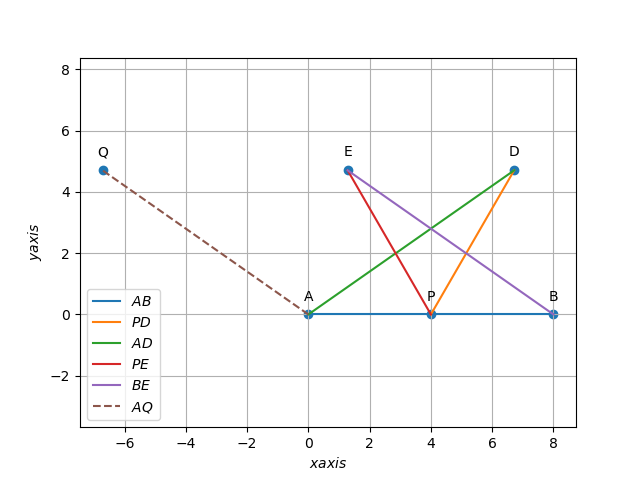
\includegraphics[width = \columnwidth]{chapters/11/10/1/14/figs/fig.png}
\caption{}
\label{fig:chapters/11/10/1/14/1}
\end{figure}
\solution
\iffalse
\documentclass[journal,12pt,twocolumn]{IEEEtran}
\usepackage{setspace}
\usepackage{gensymb}
\singlespacing
\usepackage[cmex10]{amsmath}
\usepackage{amsthm}
\usepackage{mathrsfs}
\usepackage{txfonts}
\usepackage{stfloats}
\usepackage{bm}
\usepackage{cite}
\usepackage{cases}
\usepackage{subfig}
\usepackage{longtable}
\usepackage{multirow}
\usepackage{enumitem}
\usepackage{mathtools}
\usepackage{steinmetz}
\usepackage{tikz}
\usepackage{circuitikz}
\usepackage{verbatim}
\usepackage{tfrupee}
\usepackage[breaklinks=true]{hyperref}
\usepackage{tkz-euclide}
\usetikzlibrary{calc,math}
\usepackage{listings}
    \usepackage{color}                                            %%
    \usepackage{array}                                            %%
    \usepackage{longtable}                                        %%
    \usepackage{calc}                                             %%
    \usepackage{multirow}                                         %%
    \usepackage{hhline}                                           %%
    \usepackage{ifthen}                                           %%
  %optionally (for landscape tables embedded in another document): %%
    \usepackage{lscape}     
\usepackage{multicol}
\usepackage{chngcntr}
\DeclareMathOperator*{\Res}{Res}
\renewcommand\thesection{\arabic{section}}
\renewcommand\thesubsection{\thesection.\arabic{subsection}}
\renewcommand\thesubsubsection{\thesubsection.\arabic{subsubsection}}

\renewcommand\thesectiondis{\arabic{section}}
\renewcommand\thesubsectiondis{\thesectiondis.\arabic{subsection}}
\renewcommand\thesubsubsectiondis{\thesubsectiondis.\arabic{subsubsection}}

% correct bad hyphenation here
\hyphenation{op-tical net-works semi-conduc-tor}
\def\inputGnumericTable{}                                 %%

\lstset{
frame=single, 
breaklines=true,
columns=fullflexible
}

\begin{document}


\newtheorem{theorem}{Theorem}[section]
\newtheorem{problem}{Problem}
\newtheorem{proposition}{Proposition}[section]
\newtheorem{lemma}{Lemma}[section]
\newtheorem{corollary}[theorem]{Corollary}
\newtheorem{example}{Example}[section]
\newtheorem{definition}[problem]{Definition}
\newcommand{\BEQA}{\begin{eqnarray}}
\newcommand{\EEQA}{\end{eqnarray}}
\newcommand{\define}{\stackrel{\triangle}{=}}

\bibliographystyle{IEEEtran}
\providecommand{\mbf}{\mathbf}
\providecommand{\pr}[1]{\ensuremath{\Pr\left(#1\right)}}
\providecommand{\qfunc}[1]{\ensuremath{Q\left(#1\right)}}
\providecommand{\sbrak}[1]{\ensuremath{{}\left[#1\right]}}
\providecommand{\lsbrak}[1]{\ensuremath{{}\left[#1\right.}}
\providecommand{\rsbrak}[1]{\ensuremath{{}\left.#1\right]}}
\providecommand{\brak}[1]{\ensuremath{\left(#1\right)}}
\providecommand{\lbrak}[1]{\ensuremath{\left(#1\right.}}
\providecommand{\rbrak}[1]{\ensuremath{\left.#1\right)}}
\providecommand{\cbrak}[1]{\ensuremath{\left\{#1\right\}}}
\providecommand{\lcbrak}[1]{\ensuremath{\left\{#1\right.}}
\providecommand{\rcbrak}[1]{\ensuremath{\left.#1\right\}}}
\theoremstyle{remark}
\newtheorem{rem}{Remark}
\newcommand{\sgn}{\mathop{\mathrm{sgn}}}
\providecommand{\abs}[1]{\left\vert#1\right\vert}
\providecommand{\res}[1]{\Res\displaylimits_{#1}} 
\providecommand{\norm}[1]{\left\lVert#1\right\rVert}
\providecommand{\mtx}[1]{\mathbf{#1}}
\providecommand{\mean}[1]{E\left[ #1 \right]}
\providecommand{\fourier}{\overset{\mathcal{F}}{ \rightleftharpoons}}
\providecommand{\system}{\overset{\mathcal{H}}{ \longleftrightarrow}}
\newcommand{\solution}{\noindent \textbf{Solution: }}
\newcommand{\cosec}{\,\text{cosec}\,}
\providecommand{\dec}[2]{\ensuremath{\overset{#1}{\underset{#2}{\gtrless}}}}
\newcommand{\myvec}[1]{\ensuremath{\begin{pmatrix}#1\end{pmatrix}}}
\newcommand{\mydet}[1]{\ensuremath{\begin{vmatrix}#1\end{vmatrix}}}
\numberwithin{equation}{subsection}
\makeatletter
\@addtoreset{figure}{problem}
\makeatother

\let\StandardTheFigure\thefigure
\let\vec\mathbf
\renewcommand{\thefigure}{\theproblem}



\def\putbox#1#2#3{\makebox[0in][l]{\makebox[#1][l]{}\raisebox{\baselineskip}[0in][0in]{\raisebox{#2}[0in][0in]{#3}}}}
     \def\rightbox#1{\makebox[0in][r]{#1}}
     \def\centbox#1{\makebox[0in]{#1}}
     \def\topbox#1{\raisebox{-\baselineskip}[0in][0in]{#1}}
     \def\midbox#1{\raisebox{-0.5\baselineskip}[0in][0in]{#1}}

\vspace{3cm}


\title{Assignment 1}
\author{Jaswanth Chowdary Madala}





% make the title area
\maketitle

\newpage

%\tableofcontents

\bigskip

\renewcommand{\thefigure}{\theenumi}
\renewcommand{\thetable}{\theenumi}


\begin{enumerate}
		\fi

Given the points
\begin{align}
\vec{A} \myvec{1985\\92},
\vec{B} \myvec{1995 \\97}
\end{align}

The direction vector is given by, 
\begin{align}
\vec{m} &= \vec{B} - \vec{A}\\
 &= \myvec{2 \\ 1}
\end{align}
The slope of the line is then obtained as 
\begin{align}
m &= \frac{1}{2}
\end{align}
The normal of the line  is given by,
\begin{align}
\vec{n} &= \myvec{1\\ -2}
\end{align}
Any point, $\vec{x}$ on the line can be written as
\begin{align}
\vec{n}^{\top} (\vec{x} -\vec{A}) &= 0 \\
\implies 
\myvec{1& -2} \vec{x} &= 1801
\end{align}
We need to find the population in the year 2010.  For
\begin{align}
\vec{x} &= \myvec{2010\\y} \\
\myvec{1&-2} \myvec{2010\\y} &= 1801 \\
\implies y &= \frac{209}{2}
\end{align}





\item Find a vector of magnitude 5 units, and parallel to the resultant of the vectors $\vec{a}=2\hat{i}+3\hat{j}-\hat{k}$ and $\vec{b}=\hat{i}-2\hat{j}+\hat{k}$.\\
\end{enumerate}
